\documentclass[conference]{IEEEtran}
\usepackage{graphicx,booktabs,amsmath,amssymb,hyperref,url,multirow}
\graphicspath{{figures/}}
\hypersetup{colorlinks=true,linkcolor=blue,urlcolor=blue,citecolor=blue}

\begin{document}

\title{RestoreLab: Universal, Hard-Routed and Soft Mixture-of-Experts Image Restoration and Style-Conditioned Face-to-Sketch Generation}

\author{\IEEEauthorblockN{Abdullah}
\IEEEauthorblockA{Generative AI --- Assignment 1\\
Code: \url{https://github.com/Abdullah8168/GenAI-Assignment1}\\
Demo video: \url{<YOUTUBE-LINK>}\\
Trained models (ONNX): \url{<GOOGLE-DRIVE-LINK-TO-outputs.zip>}}}

\maketitle

\begin{abstract}
We design, train, evaluate and deploy four generative systems. Tasks 1--3 restore 128$\times$128 Oxford-IIIT Pet images corrupted at runtime by salt-and-pepper noise, Gaussian blur or rectangular occlusion: (1) a single universal denoising autoencoder (DAE) with a compressed latent bottleneck, (2) a corruption classifier that hard-routes inputs to three specialist DAEs with an identity bypass for clean images, and (3) a differentiable soft mixture-of-experts (MoE) initialised from the Task~2 models and fine-tuned jointly with reconstruction, SSIM, classification and routing-balance losses. Task~4 is a style-conditioned pix2pix-style conditional GAN (U-Net generator, PatchGAN discriminator, learned style embeddings) trained on FS2K. All hyper-parameters are tuned with Optuna, experiments are tracked in MLflow, all inference models are exported to ONNX and verified against PyTorch, and the system is served by a FastAPI backend and a React/Tailwind frontend started with a single Docker Compose command.
\end{abstract}

\begin{IEEEkeywords}
denoising autoencoder, mixture of experts, conditional GAN, Optuna, ONNX, image restoration
\end{IEEEkeywords}

%=====================================================================
\section{Introduction}
Real images are degraded in heterogeneous ways, and a restoration system rarely knows which degradation it faces. We compare three answers to this problem: one universal model (Task~1), explicit classification followed by specialists (Task~2), and a learned soft combination of specialists (Task~3). Task~4 studies paired image-to-image translation with an explicit categorical style condition. The emphasis is a complete pipeline: reproducible data generation, hyper-parameter search, tracked experiments, verified model export and a containerised application.

\section{Related Work}
Denoising autoencoders learn robust representations by reconstructing clean inputs from corrupted ones~\cite{vincent2008}. Encoder--decoder CNNs such as U-Net~\cite{unet} are the standard backbone for restoration; skip connections improve detail but can bypass the bottleneck, which is why our autoencoders avoid unrestricted skips (Sec.~\ref{sec:t1}). SSIM~\cite{ssim} complements $L_1$ by measuring local structure, and combinations of $L_1$ and SSIM were shown to outperform $L_2$ for restoration~\cite{zhao2017}. Mixture-of-experts models~\cite{jacobs1991} combine specialists through a gating network; sparse MoEs add load-balancing losses to prevent expert collapse~\cite{shazeer2017,switch}, which motivates our balance regulariser. Conditional GANs for paired translation (pix2pix)~\cite{pix2pix} use a U-Net generator and a PatchGAN discriminator with an $L_1$ term ($\lambda=100$). FS2K~\cite{fs2k} provides 2{,}104 photo--sketch pairs in three styles. Optuna~\cite{optuna} provides TPE sampling and median pruning.

%=====================================================================
\section{Data Preparation}
\subsection{Oxford-IIIT Pet (Tasks 1--3)}
The official trainval list (3{,}680 images) is split 80/20 with seed 42 into 2{,}944 training and 736 validation images; the official test list (3{,}669 images) is used only for final evaluation. Images are converted to RGB and resized to 128$\times$128 (bicubic) and cached once as a \texttt{uint8} array. Because the official Oxford server repeatedly stalled during the download on Colab, images were loaded from the \texttt{timm/oxford-iiit-pet} mirror, which preserves the official splits and file names; images are ordered by file name so the split is independent of the source.

\subsection{Runtime corruption pipeline}
Corruptions are generated in the data loader every time an image is loaded; no corrupted copies are stored. Each training image receives one of four conditions with probability $1/4$ (Table~\ref{tab:corr}). Salt-and-pepper noise selects each pixel with probability $p$ and sets it to black or white with equal probability (identically in all three channels). Blur uses a separable Gaussian kernel with reflect padding (same construction as \texttt{torchvision}). Occlusion splits a target area between 1--3 rectangles with a Dirichlet draw, samples aspect ratios in $[0.5,2]$ and random positions, and re-samples until the measured \emph{union} lies within $\pm0.5\%$ of the target; this was introduced after a test showed overlapping rectangles produced only 8.7\% coverage. The corruption module is pure NumPy and is copied unchanged into the backend container, so the application applies exactly the training corruptions.

\begin{table}[t]
\caption{Corruption configuration}\label{tab:corr}
\centering\footnotesize
\begin{tabular}{@{}p{1.45cm}p{3.1cm}p{2.9cm}@{}}
\toprule
Condition & Training (random) & Test (low / med / high)\\\midrule
Clean & original image & original image\\
Salt \& pepper & $p\sim U(0.02,0.15)$ & $p=0.03/0.08/0.15$\\
Gaussian blur & $k\in\{3,5,7\}$, $\sigma\sim U(0.5,2.5)$ & $(3,0.7)/(5,1.5)/(7,2.5)$\\
Occlusion & 1--3 black rectangles, union 10--35\% & 10/20/35\% with 1/2/3 rects\\
\bottomrule
\end{tabular}
\end{table}

\textbf{Manifests.} Validation and test corruptions are deterministic. A validation manifest assigns exactly balanced conditions to the 736 validation images; the test manifest contains, for each of the 3{,}669 test images, one clean entry and the nine fixed (type, severity) entries (36{,}690 entries). Each entry stores type, severity, parameters, rectangle coordinates and the seed.

\subsection{FS2K (Task 4)}
The official FS2K train/test annotation files define the split. 15\% of the official training pairs are held out for validation, stratified by style with seed 42. Photos and sketches are resized to 128$\times$128 and normalised to $[-1,1]$. Augmentation (resize to 142, random 128 crop, horizontal flip) is applied to the photo and sketch \emph{concatenated along the channel axis}, guaranteeing identical spatial transforms and preserving pixel correspondence.

%=====================================================================
\section{Task 1: Universal Denoising Autoencoder}\label{sec:t1}
\subsection{Architecture}
The encoder has four stages (128$\rightarrow$64$\rightarrow$32$\rightarrow$16$\rightarrow$8), each a stride-2 4$\times$4 convolution and a 3$\times$3 convolution with BatchNorm and LeakyReLU; channels grow $b,2b,4b,8b$. A 1$\times$1 convolution compresses the 8$\times$8 feature map to $z$ channels, giving a latent of $64z$ values (e.g. $z{=}16$: 1{,}024 values versus 49{,}152 input values, a 48$\times$ compression); dropout is applied to the latent. The decoder mirrors the encoder using nearest-neighbour upsampling followed by 3$\times$3 convolutions (avoiding checkerboard artefacts of transposed convolutions) and a sigmoid output. The submitted model has \emph{no skip connections}; an ablation adds one skip at 64$\times$64 (Table~\ref{tab:t1abl}).

\subsection{Loss and Optuna search}
$\mathcal{L}=\alpha\,\mathcal{L}_{1}(x,\hat x)+(1-\alpha)\,(1-\mathrm{SSIM}(x,\hat x))$ with SSIM computed with an 11$\times$11 Gaussian window ($\sigma=1.5$). The validation objective is $0.5\,\mathrm{SSIM}+0.5\,\mathrm{PSNR}/40$. Search space: learning rate $[10^{-4},3\cdot10^{-3}]$ (log), batch $\{32,64,128\}$, $z\in\{8,16,32\}$, base channels $b\in\{16,32,48\}$, dropout $[0,0.3]$, $\alpha\in[0.5,0.95]$; TPE sampler (seed 42), median pruner, 12 trials of 5 epochs. The best configuration was retrained for 40 epochs with AdamW and cosine decay.

Of the 12 trials, 3 completed and 9 were pruned by the median pruner. The best trial (\#1, score 0.509) selected lr $=1.70\cdot10^{-3}$, batch 32, $z=16$ (latent 1{,}024), $b=32$, dropout 0.088 and $\alpha=0.665$, i.e. Optuna moved toward the SSIM term relative to the suggested $\alpha=0.8$ (Fig.~\ref{fig:t1hist}).
\begin{figure}[t]\centering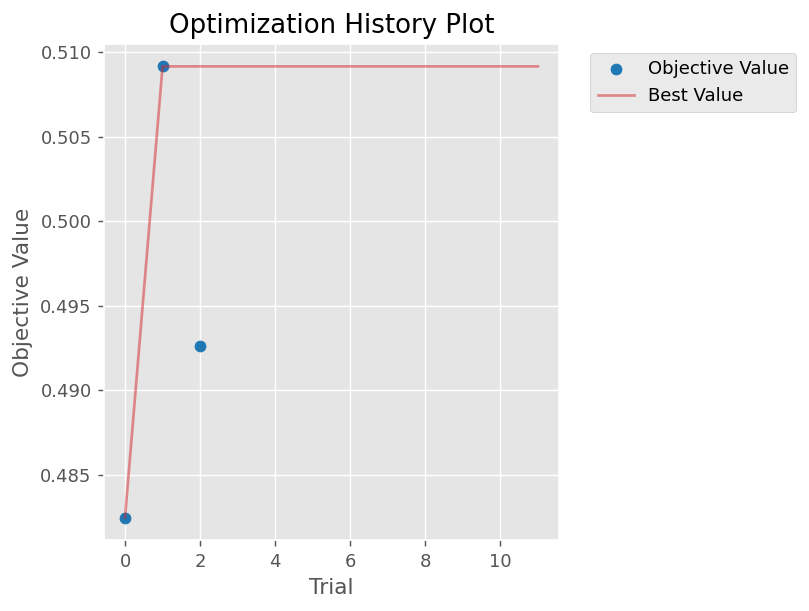
\includegraphics[width=\columnwidth]{task1_universal_dae_history}\caption{Task 1 Optuna optimisation history.}\label{fig:t1hist}\end{figure}


\subsection{Results}
Table~\ref{tab:t1} reports test PSNR/SSIM per corruption and severity next to the score of the corrupted input. The universal DAE produces an almost constant output quality ($\approx$21~dB, SSIM 0.66--0.69) irrespective of the input: it strongly improves salt-and-pepper inputs (+5.0~dB, SSIM 0.38$\rightarrow$0.68) and occlusions (+5.8~dB), but it \emph{degrades} clean and mildly blurred inputs (clean SSIM 1.00$\rightarrow$0.69; low blur 32.3$\rightarrow$21.5~dB). This is the cost of a genuine bottleneck: every image is re-synthesised from a 1{,}024-value code, which removes fine texture regardless of the corruption. Error maps (Fig.~\ref{fig:t1ex}) concentrate on fur texture and edges; failure cases (Fig.~\ref{fig:t1fail}) are large high-severity occlusions, where hidden content must be hallucinated and is filled with blurry average colour.

\textbf{Skip-connection ablation.} With identical hyper-parameters and 15 epochs, a single skip connection at 64$\times$64 raised clean-image PSNR from 20.8 to 32.3~dB and salt PSNR from 20.7 to 28.3~dB (Table~\ref{tab:t1abl}). The skip transmits high-frequency detail around the bottleneck, explaining the gain, but it also gives the network a route to copy corruption, which is why unrestricted skips are not allowed. We submit the skip-free model as the genuine autoencoder and report the ablation as evidence of the trade-off.

\begin{table}[t]\caption{Task 1 test results (input $\rightarrow$ output)}\label{tab:t1}\centering\footnotesize
\begin{tabular}{@{}llcccc@{}}\toprule
Type & Sev. & PSNR in & PSNR out & SSIM in & SSIM out\\\midrule
Clean & -- & $\infty$ & 21.45 & 1.000 & 0.691\\
Salt & low & 20.14 & 21.45 & 0.603 & 0.688\\
 & med & 15.88 & 21.42 & 0.340 & 0.682\\
 & high & 13.14 & 21.36 & 0.204 & 0.672\\
Blur & low & 32.34 & 21.51 & 0.944 & 0.690\\
 & med & 26.77 & 21.45 & 0.806 & 0.679\\
 & high & 24.35 & 21.09 & 0.692 & 0.648\\
Occl. & low & 16.63 & 20.39 & 0.862 & 0.655\\
 & med & 13.32 & 19.51 & 0.728 & 0.618\\
 & high & 10.75 & 18.27 & 0.540 & 0.561\\\midrule
All & & -- & 20.79 & 0.672 & 0.659\\\bottomrule\end{tabular}\end{table}

\begin{table}[t]\caption{Skip-connection ablation (test PSNR / SSIM, 15 epochs)}\label{tab:t1abl}\centering\footnotesize
\begin{tabular}{@{}lcc@{}}\toprule
Input & No skip & One skip (64$\times$64)\\\midrule
Clean & 20.83 / 0.635 & 32.26 / 0.954\\
Salt & 20.70 / 0.617 & 28.31 / 0.852\\
Blur & 20.78 / 0.622 & 27.70 / 0.823\\
Occlusion & 18.81 / 0.565 & 21.68 / 0.781\\\bottomrule\end{tabular}\end{table}
\begin{figure}[t]\centering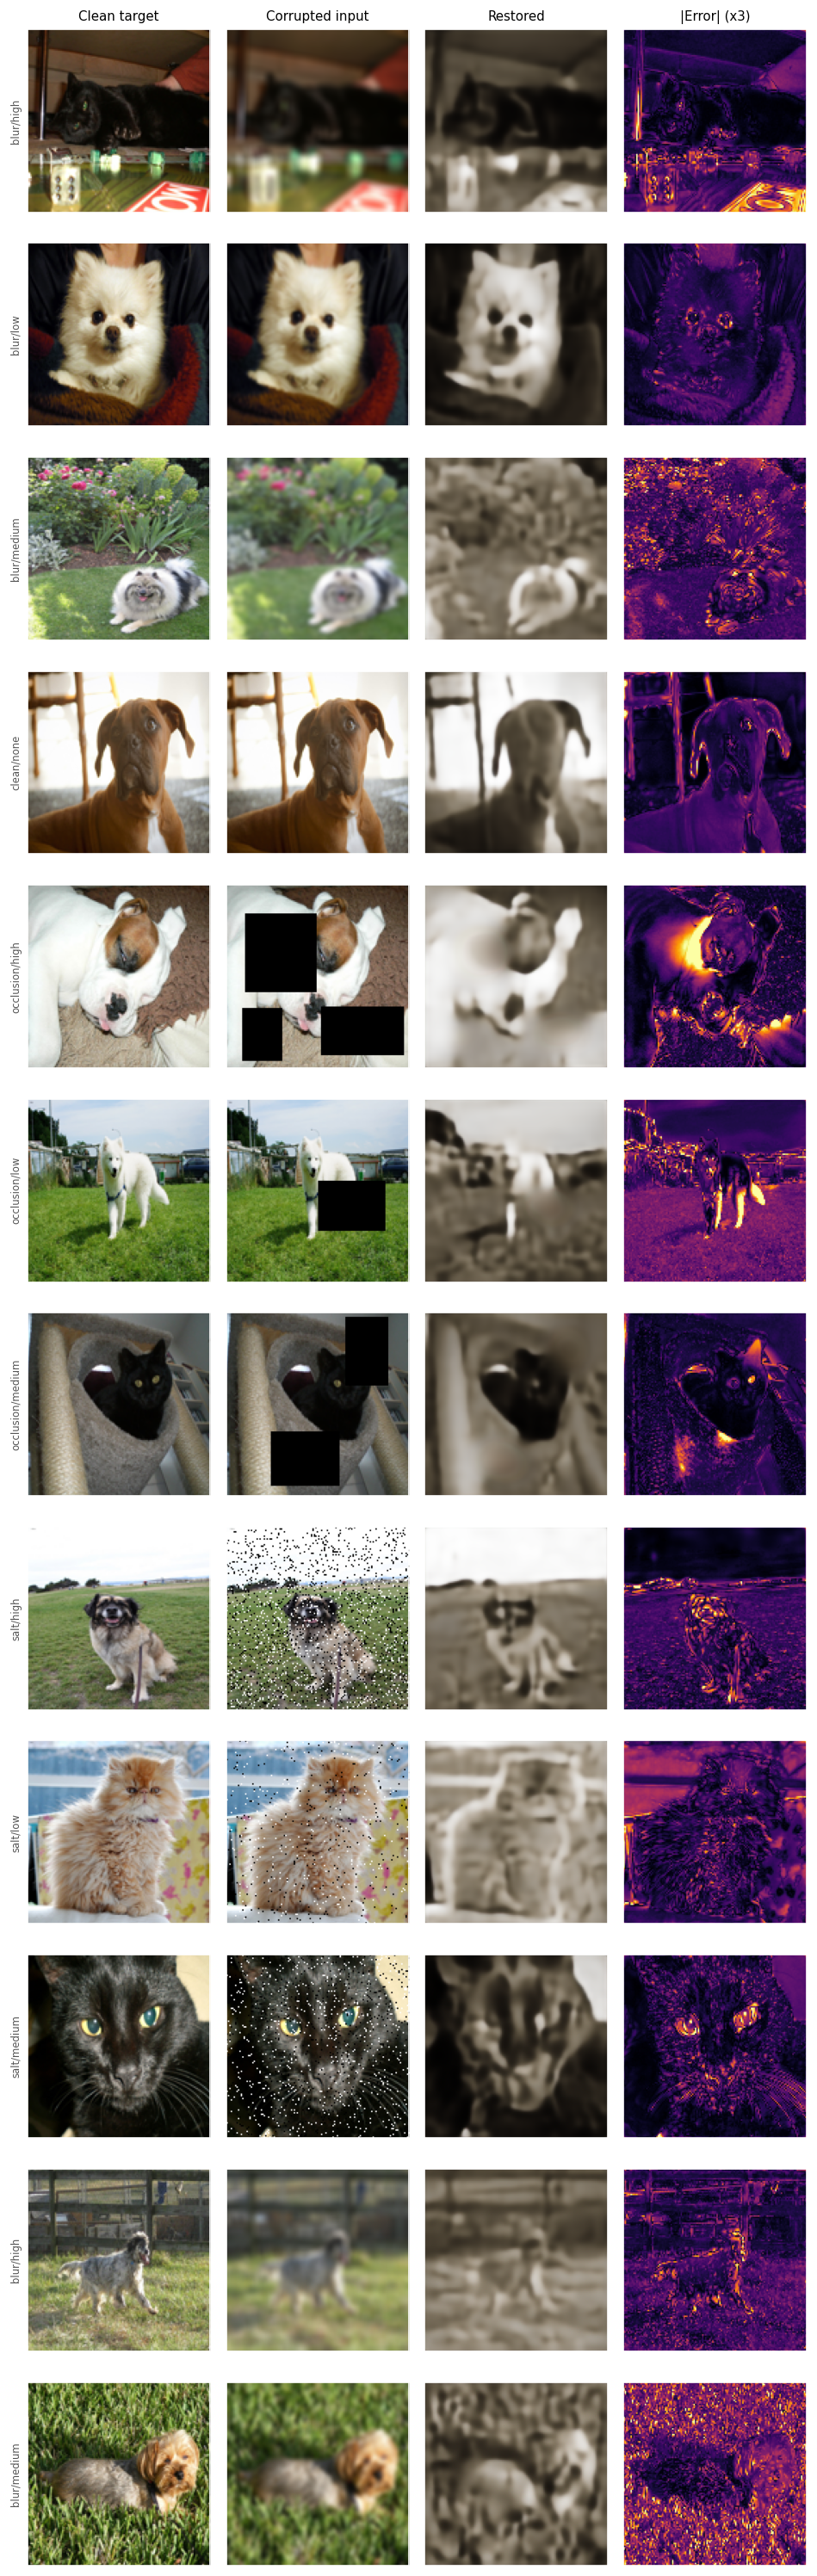
\includegraphics[width=\columnwidth]{task1_examples}\caption{Task 1 test examples: clean target, corrupted input, reconstruction, absolute error map ($\times$3).}\label{fig:t1ex}\end{figure}
\begin{figure}[t]\centering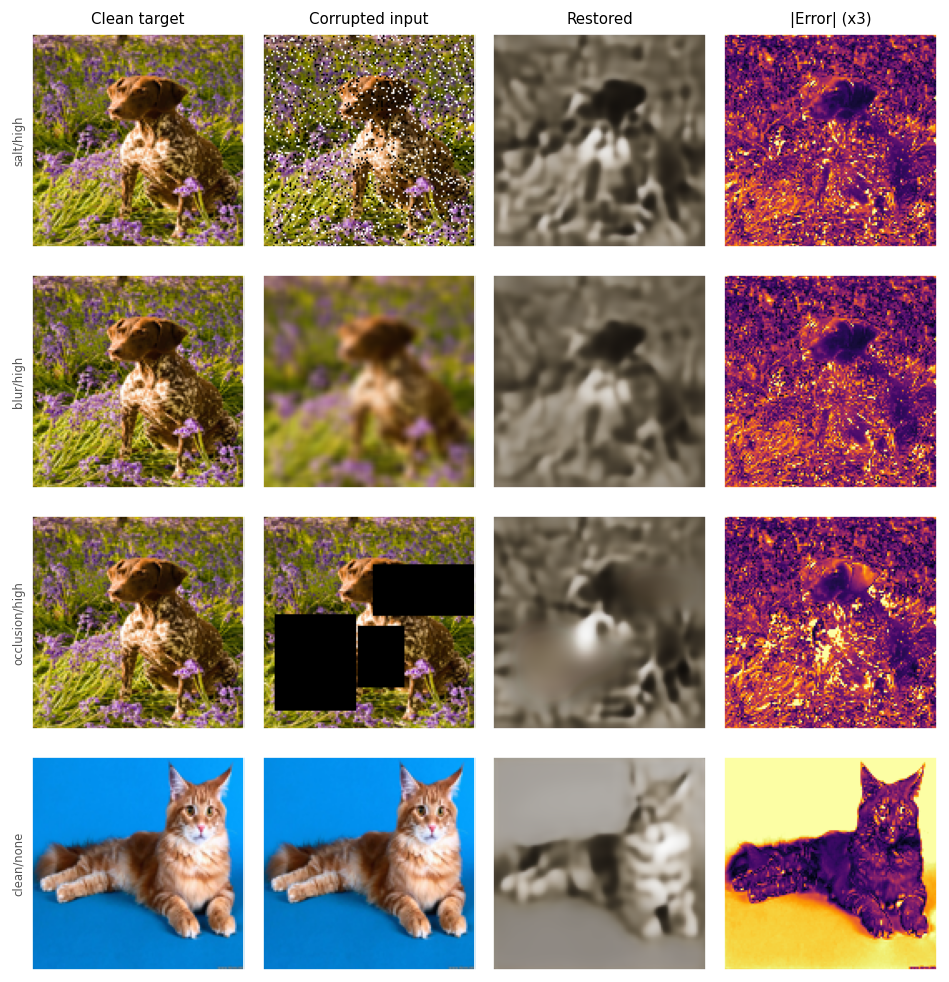
\includegraphics[width=\columnwidth]{task1_failures}\caption{Task 1 failure cases (worst SSIM per corruption and lowest PSNR gain).}\label{fig:t1fail}\end{figure}
\begin{figure}[t]\centering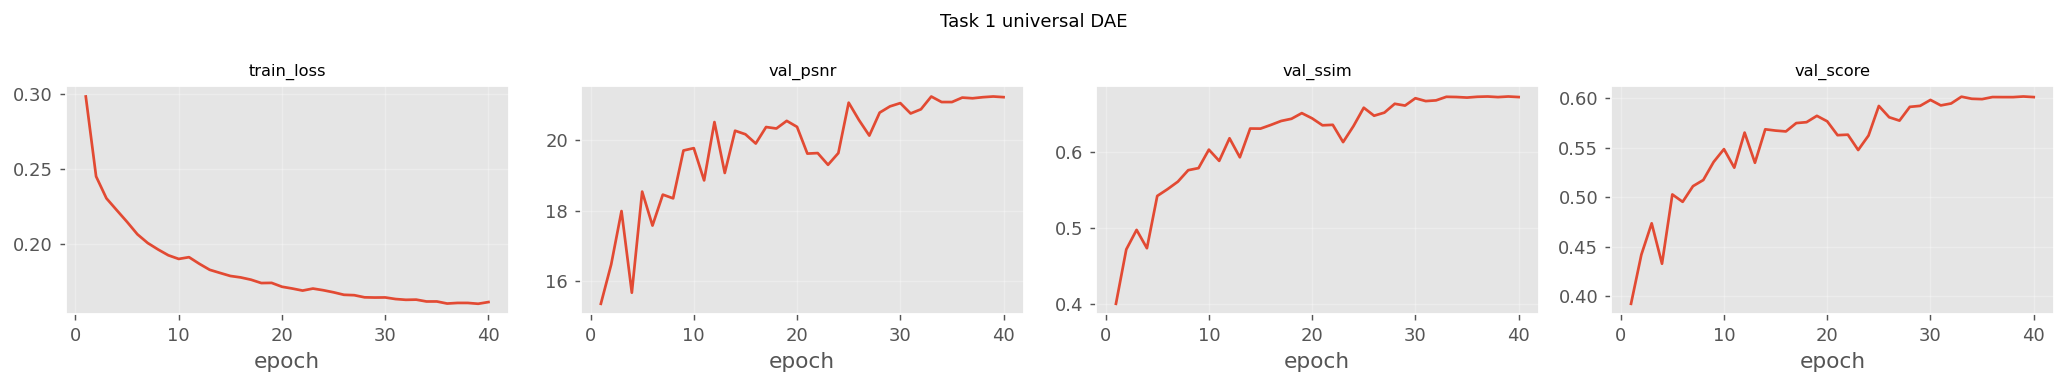
\includegraphics[width=\columnwidth]{task1_curves}\caption{Task 1 training loss and validation PSNR/SSIM.}\label{fig:t1curve}\end{figure}


%=====================================================================
\section{Task 2: Classification and Hard-Routed Specialists}
\subsection{Classifier}
A four-stage CNN (two 3$\times$3 conv--BN--ReLU layers and max-pooling per stage, channels $b,2b,4b,8b$, global average pooling, dropout, linear layer) predicts clean/salt/blur/occlusion. The first stage keeps full resolution because blur and impulse noise are high-frequency cues. A custom batch sampler forces exactly $B/4$ samples of each class into every batch. Optuna tuned learning rate, batch size, channels, dropout and weight decay (10 trials of 4 epochs; objective: validation macro-F1).

\subsection{Specialists and routing}
Three DAEs with the Task~1 architecture are trained only on their own corruption. A shared Optuna search (8 trials; each trial trains all three for 4 epochs, objective = mean validation score) selects one architecture (learning rate, batch, $z$, channels, $\alpha$); the three specialists are then trained independently with different seeds. At inference, $r=\arg\max_k p_k$ selects the specialist, and clean inputs are returned unchanged (identity bypass). We evaluate \emph{oracle} routing (true label selects the expert) and \emph{predicted} routing.

\subsection{Results}
\textbf{Classifier.} Optuna (4 completed, 6 pruned trials) selected lr $8.3\cdot10^{-4}$, batch 32, $b=32$, dropout 0.44 and weight decay $7.7\cdot10^{-5}$ (validation macro-F1 0.992). On the 36{,}690 test inputs the classifier reaches \textbf{99.52\% accuracy}, macro precision 0.992, recall 0.993 and \textbf{macro-F1 0.992}; per-class F1 is 0.977 (clean), 0.9995 (salt), 0.997 (blur) and 0.995 (occlusion). Every medium- and high-severity input is classified correctly; all errors occur at the lowest severities (Fig.~\ref{fig:cm}): 88 low occlusions (10\% area) and 10 low salt inputs are called \emph{clean}, and 58 clean photographs, which are naturally soft or out of focus, are called \emph{blur}.

\textbf{Specialists.} The shared search selected lr $2.7\cdot10^{-3}$, batch 32, $z=32$ (latent 2{,}048), $b=48$ and $\alpha=0.56$.

\textbf{Routing.} Oracle routing reaches 30.49~dB / SSIM 0.754 overall and predicted routing 30.35~dB / 0.754 (Table~\ref{tab:t2}). The near-identical numbers show that the operational system is limited by the specialists, not by the classifier. Specialists clearly beat the universal model on their own corruption (salt 24.2 vs 21.4~dB, blur 24.3 vs 21.3~dB) because each devotes its full capacity to one inverse problem, and the identity bypass keeps clean images intact. Misrouting costs are concentrated in clean images sent to the blur or occlusion expert (72 images needlessly smoothed) and in low occlusions sent to the identity branch, which are returned unrepaired (Fig.~\ref{fig:t2fail}). For low blur the specialist output (24.2~dB) is worse than the input (32.3~dB): the specialist's bottleneck removes more detail than the mild blur did.

\begin{table}[t]\caption{Task 2 test PSNR / SSIM: oracle vs predicted routing}\label{tab:t2}\centering\footnotesize
\begin{tabular}{@{}lccc@{}}\toprule
Type & Input & Oracle & Predicted\\\midrule
Clean & $\infty$ / 1.000 & $\infty$ / 1.000 & 98.5 / 0.996\\
Salt & 16.39 / 0.382 & 24.22 / 0.765 & 24.22 / 0.765\\
Blur & 27.82 / 0.814 & 24.32 / 0.763 & 24.33 / 0.763\\
Occlusion & 13.57 / 0.710 & 19.75 / 0.651 & 19.76 / 0.653\\\midrule
All & 27.33 / 0.672 & 30.49 / 0.754 & 30.35 / 0.754\\\bottomrule\end{tabular}\end{table}
\begin{figure}[t]\centering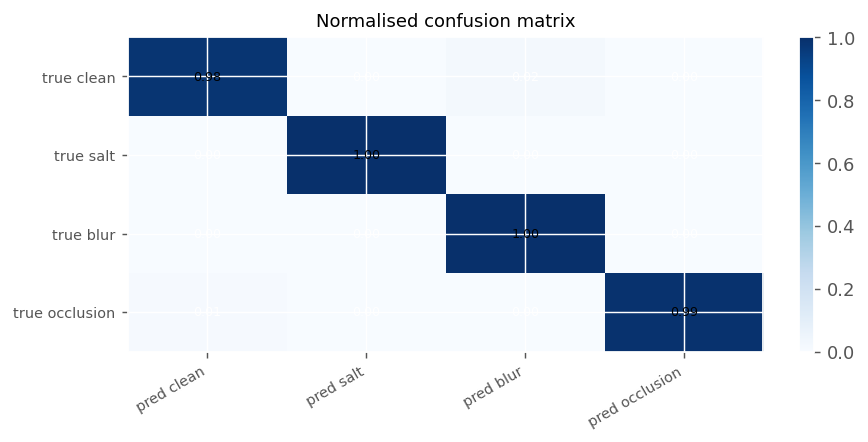
\includegraphics[width=0.85\columnwidth]{task2_classifier_test_confusion}\caption{Task 2 normalised confusion matrix on the test manifest.}\label{fig:cm}\end{figure}
\begin{figure}[t]\centering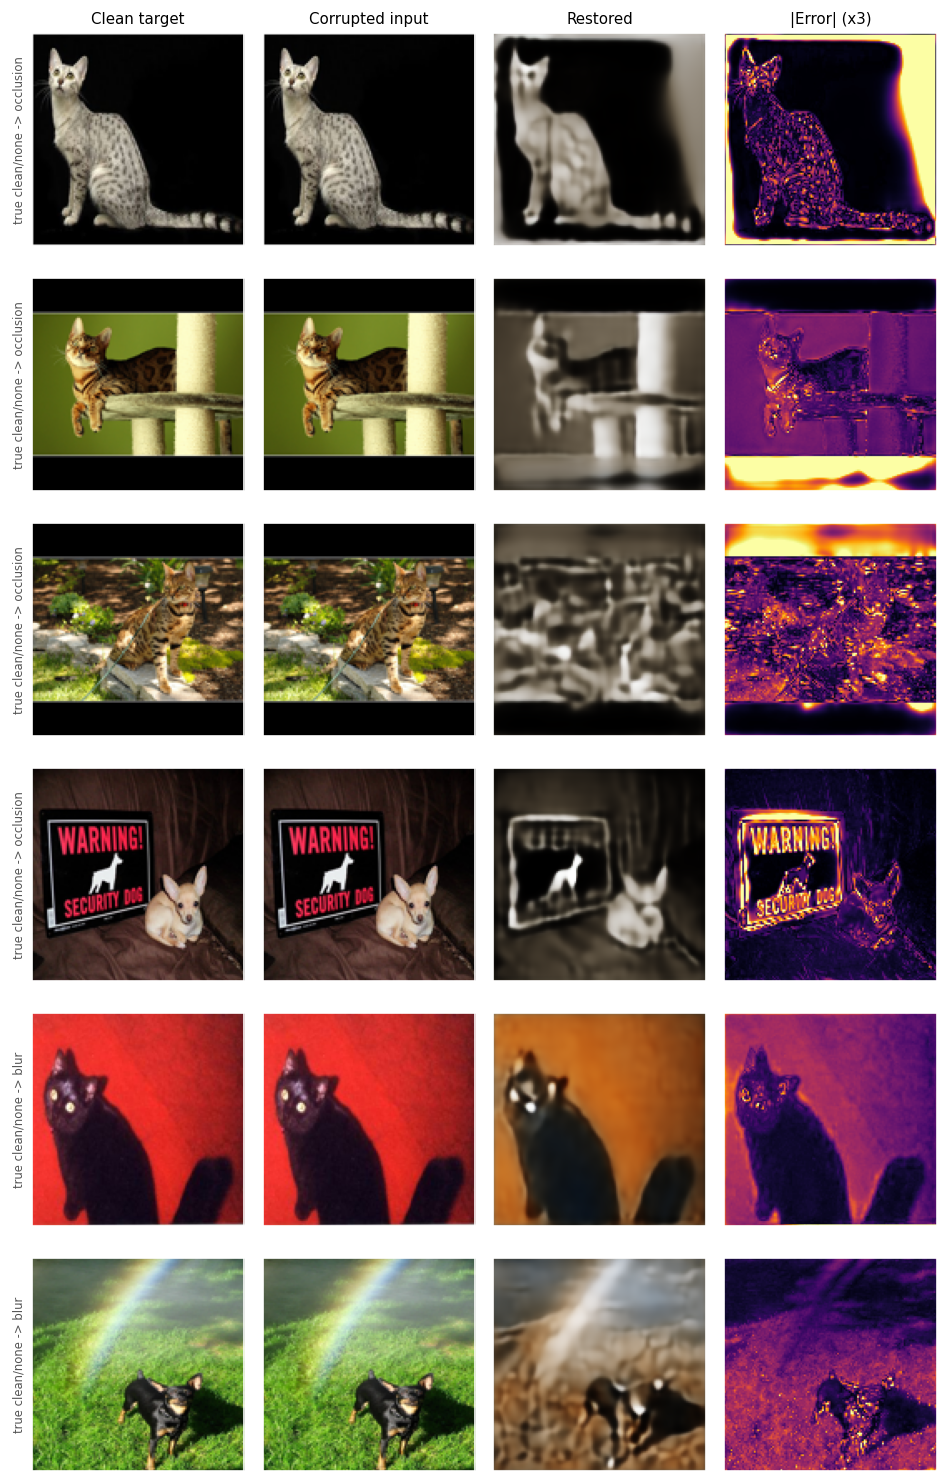
\includegraphics[width=\columnwidth]{task2_misrouting_failures}\caption{Restoration failures caused by classifier errors (true $\rightarrow$ predicted route).}\label{fig:t2fail}\end{figure}
\begin{figure}[t]\centering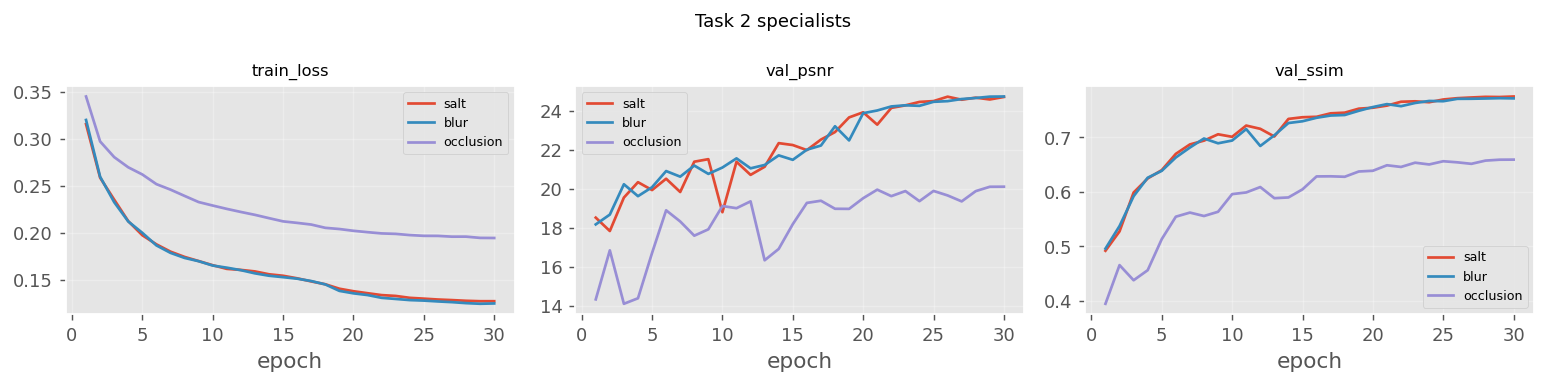
\includegraphics[width=\linewidth]{task2_specialist_curves}\caption{Training curves of the three specialists.}\label{fig:t2curve}\end{figure}


%=====================================================================
\section{Task 3: Soft Mixture-of-Experts}
\subsection{Model and training}
$w=\mathrm{softmax}(G(\tilde x)/\tau)$ weights four branches: identity, salt, blur and occlusion experts; $\hat x=w_0\tilde x+\sum_k w_k A_k(\tilde x)$. The gate is initialised from the Task~2 classifier (identical class order) and the experts from the specialists. A warm-up stage trains only the gate with experts frozen (BatchNorm statistics fixed); joint fine-tuning then unfreezes all parameters with a 10$\times$ smaller learning rate for the experts. The loss is
$\mathcal{L}=\lambda_1\mathcal{L}_1+\lambda_s(1-\mathrm{SSIM})+\lambda_c\mathcal{L}_{CE}+\lambda_b\sum_k(\bar w_k-\tfrac14)^2$, with $\lambda_s=1-\lambda_1$ and balanced batches so $\bar w_k=1/4$ is the correct target. Optuna searched the joint learning rate, $\tau\in[0.3,3]$, $\lambda_c$, $\lambda_b$ and $\lambda_1$; trials where any branch's mean validation weight fell below 2\% were pruned as routing collapse.

\subsection{Results}
Because of the deadline, Task~3 used a reduced schedule (4 Optuna trials of 1+1 epochs, then 1 warm-up and 4 joint epochs). The best trial selected joint lr $4.3\cdot10^{-5}$, $\tau=2.68$, $\lambda_c=0.29$, $\lambda_b=0.041$ and $\lambda_1=0.57$. The soft MoE obtains the best SSIM of all systems on every corruption (Table~\ref{tab:cmp}): salt 24.37 vs 24.22~dB for hard routing, blur 25.13 vs 24.33~dB, occlusion 19.99 vs 19.76~dB. Its weakness is clean images (45.5~dB instead of perfect): with $\tau=2.68$ the identity branch receives on average 0.90 of the weight for clean inputs, and the remaining 10\% blends in expert reconstructions.

\textbf{Routing behaviour.} Mean weights per true corruption (Fig.~\ref{fig:heat}) form a clear diagonal: salt inputs give the salt expert 0.95--0.97, high occlusion gives the occlusion expert 0.995, and blur gives the blur expert 0.77--0.80 while 0.16--0.18 stays on the identity branch, which is reasonable because a blurred input is already close to its target. Weights are most distributed for low-severity inputs (low occlusion: identity 0.18, occlusion 0.77). No expert is inactive (mean weights 0.16/0.30/0.24/0.29), no branch dominates unrelated inputs (mean weight on inputs it is not responsible for $\le$0.023 for the experts and 0.083 for identity), the arg-max route matches the true label for 99.3\% of inputs, and the mean routing entropy is 0.36 nats (maximum 1.39).

\textbf{Mixed corruptions.} On 300 test images with two simultaneous medium corruptions (outside the training distribution), soft routing beat hard routing in all three combinations (salt+blur 22.50 vs 21.92~dB; blur+occlusion 19.91 vs 19.87~dB; salt+occlusion 14.52 vs 13.54~dB), confirming that blending experts helps when no single class is correct. For salt+occlusion the universal DAE was best (19.89~dB): routing chose the salt expert (weight 0.87) and left the occluded region unfilled.

\begin{table}[t]\caption{Comparison of all systems (test PSNR / SSIM)}\label{tab:cmp}\centering\footnotesize
\begin{tabular}{@{}lcccc@{}}\toprule
Type & Universal & Hard (pred.) & Hard (oracle) & Soft MoE\\\midrule
Clean & 21.45/.691 & 98.5/.996 & $\infty$/1.00 & 45.46/.995\\
Salt & 21.41/.681 & 24.22/.765 & 24.22/.765 & \textbf{24.37/.771}\\
Blur & 21.35/.672 & 24.33/.763 & 24.32/.763 & \textbf{25.13/.782}\\
Occl. & 19.39/.611 & 19.76/.653 & 19.75/.651 & \textbf{19.99/.675}\\\bottomrule\end{tabular}\end{table}
\begin{figure}[t]\centering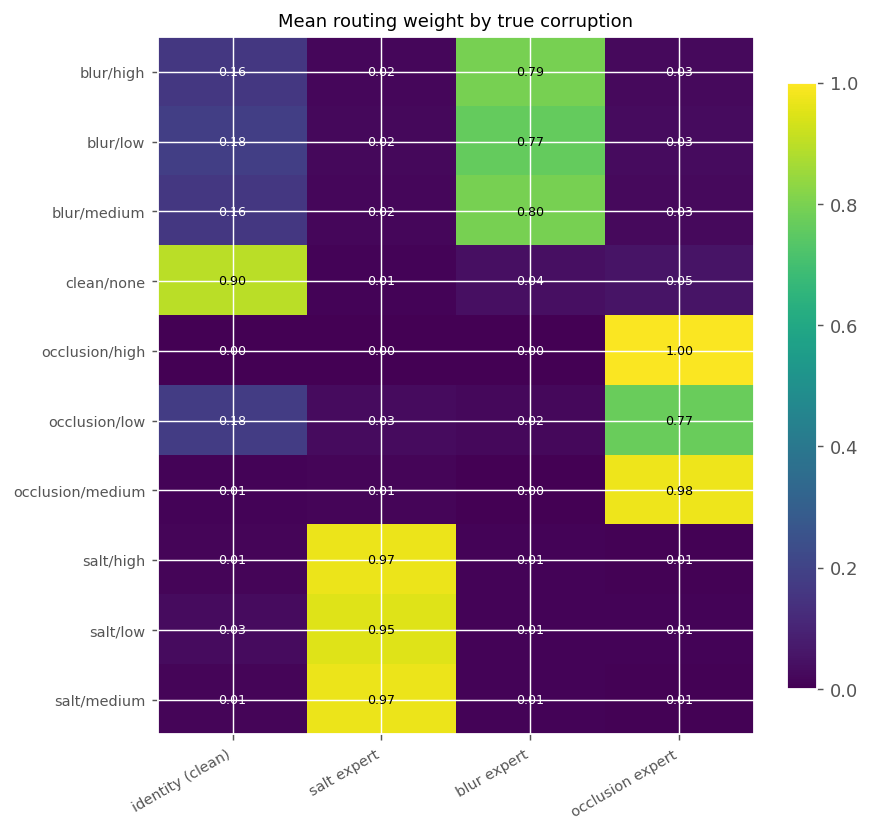
\includegraphics[width=\columnwidth]{task3_routing_heatmap}\caption{Task 3 routing heatmap: mean branch weight for each true corruption and severity.}\label{fig:heat}\end{figure}
\begin{figure}[t]\centering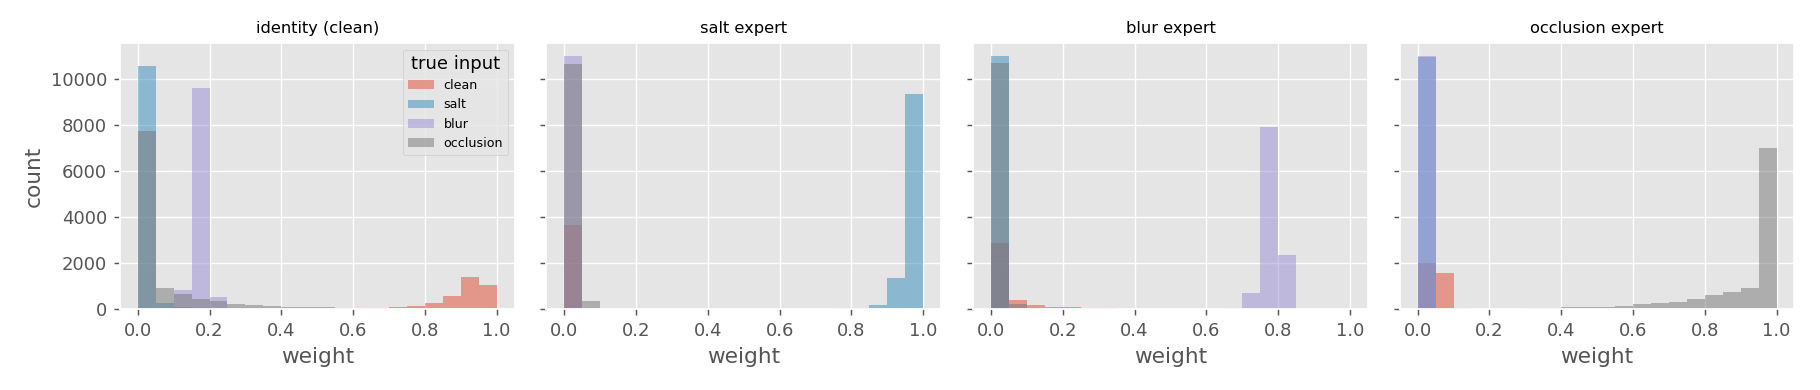
\includegraphics[width=\linewidth]{task3_weight_distribution}\caption{Distribution of routing weights per branch, coloured by true input condition.}\label{fig:wdist}\end{figure}
\begin{figure}[t]\centering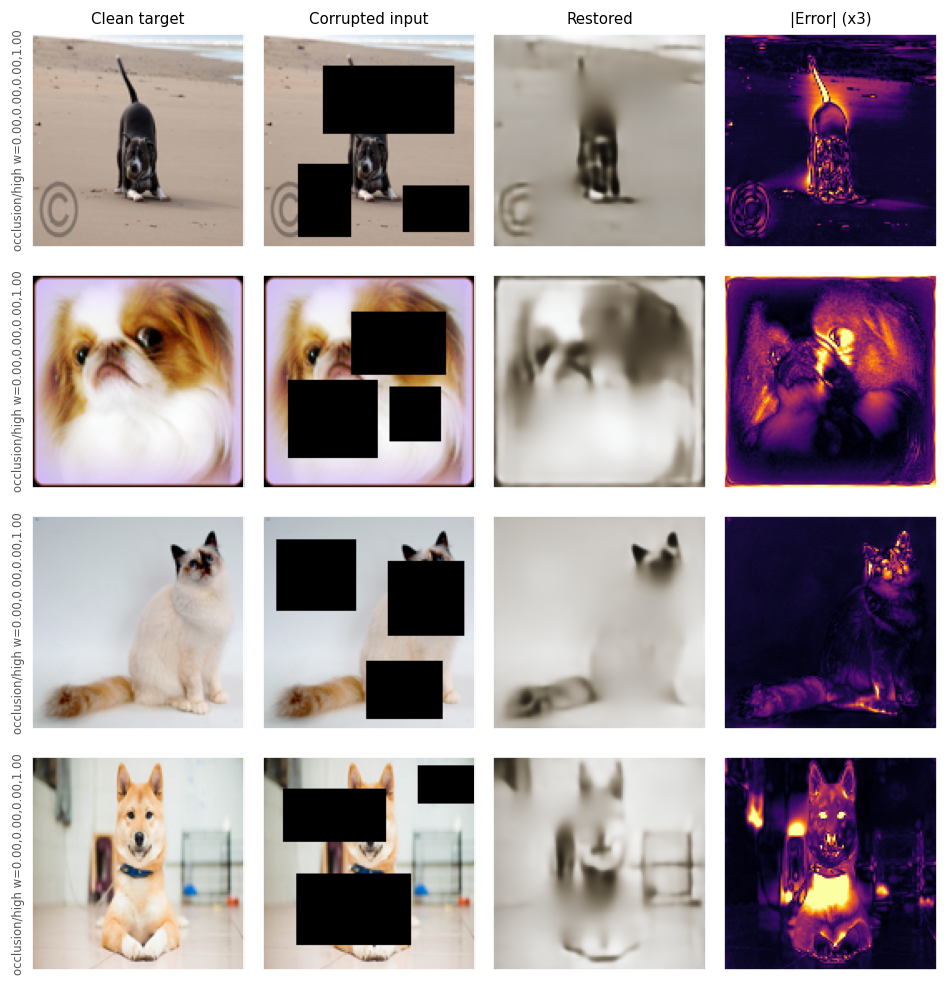
\includegraphics[width=\columnwidth]{task3_dominant_examples}\caption{Examples where one expert dominates (lowest routing entropy).}\label{fig:dom}\end{figure}
\begin{figure}[t]\centering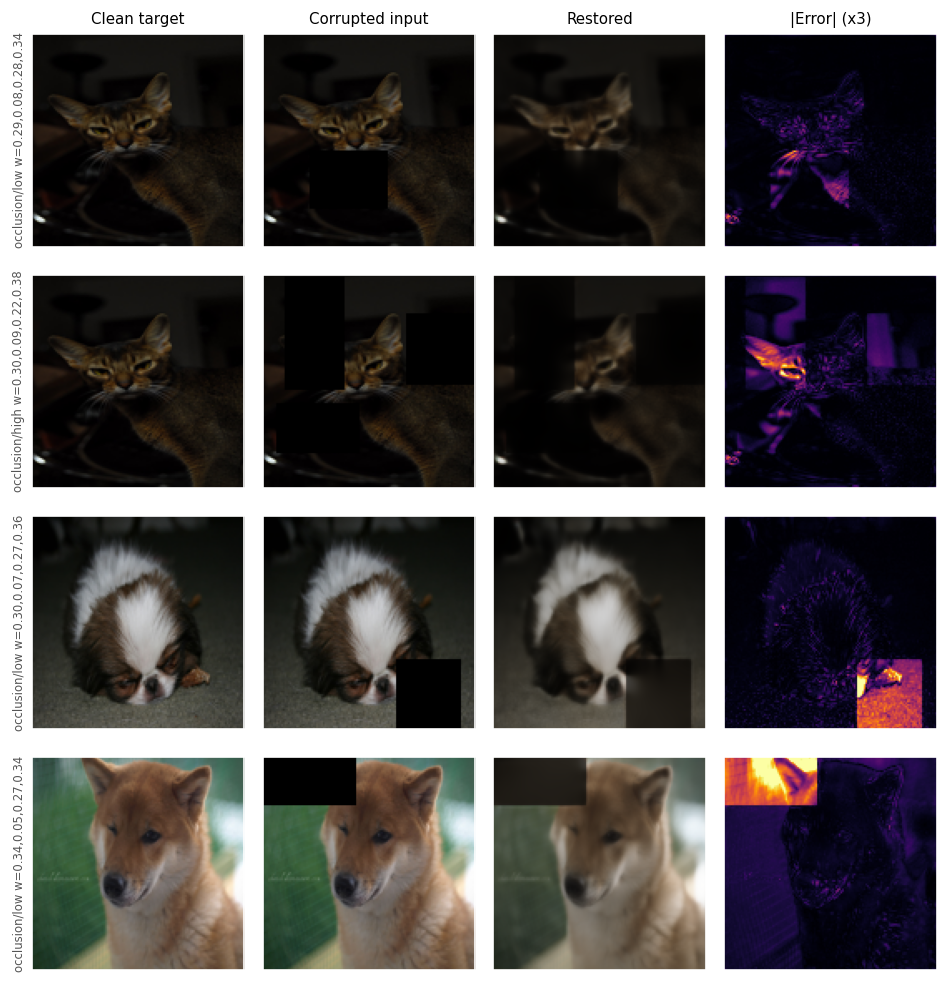
\includegraphics[width=\columnwidth]{task3_distributed_examples}\caption{Examples with distributed weights (highest routing entropy).}\label{fig:dist}\end{figure}


%=====================================================================
\section{Task 4: Style-Conditioned Face-to-Sketch cGAN}
\subsection{Architecture and losses}
The generator is a 7-level U-Net (128$\rightarrow$1) with skip connections and dropout in the first three decoder blocks. A learned \texttt{nn.Embedding}(3,$d$) style vector is tiled and concatenated with the input photo and also projected and added at the 1$\times$1 bottleneck. The PatchGAN discriminator receives photo, sketch and its own tiled style embedding and outputs a 14$\times$14 map of logits. $\mathcal{L}_D=\tfrac12[\mathrm{BCE}(D(x,y,s),1)+\mathrm{BCE}(D(x,G(x,s),s),0)]$ and $\mathcal{L}_G=\mathrm{BCE}(D(x,G(x,s),s),1)+\lambda_{L1}\|y-G(x,s)\|_1$. Adam ($\beta_1=0.5$), linear decay in the second half. Optuna tuned $lr_G$, $lr_D$, batch, base channels, dropout, embedding size and $\lambda_{L1}\in[10,200]$ with short trials (objective: validation $L_1+0.5(1-\mathrm{SSIM})$); D-real, D-fake, G-adversarial and G-$L_1$ losses are logged separately, and generated samples of the same validation photos are logged at fixed intervals.

\subsection{Results}
Task~4 used a strongly reduced schedule (2 Optuna trials of 2 epochs; final training 10 epochs), so the results demonstrate a working pipeline rather than converged quality. The selected configuration was $lr_G=1.2\cdot10^{-4}$, $lr_D=4.3\cdot10^{-4}$, batch 4, 64 base channels, dropout 0.30, embedding dimension 32 and $\lambda_{L1}=121$, close to the pix2pix value of 100. On the official test set the generator reaches $L_1$ 0.119, SSIM 0.417 and PSNR 14.85~dB overall; per style: Style~1 0.089 / 0.466 / 16.6~dB, Style~2 0.173 / 0.325 / 11.7~dB, Style~3 0.083 / 0.531 / 17.4~dB. Style~2 is clearly hardest; it is the smallest FS2K style (98 photographs), so the shared generator has seen few examples of it, a class-imbalance effect that the stratified split preserves but cannot fix. The style-control figure (Fig.~\ref{fig:style}) shows that one photograph changes appearance with the condition, confirming that the generator uses the embedding. The loss curves (Fig.~\ref{fig:t4loss}) show the discriminator and generator losses separately; after only 10 epochs the sketches are still blurry with weak hair and background detail (Fig.~\ref{fig:t4fail}).
\begin{figure}[t]\centering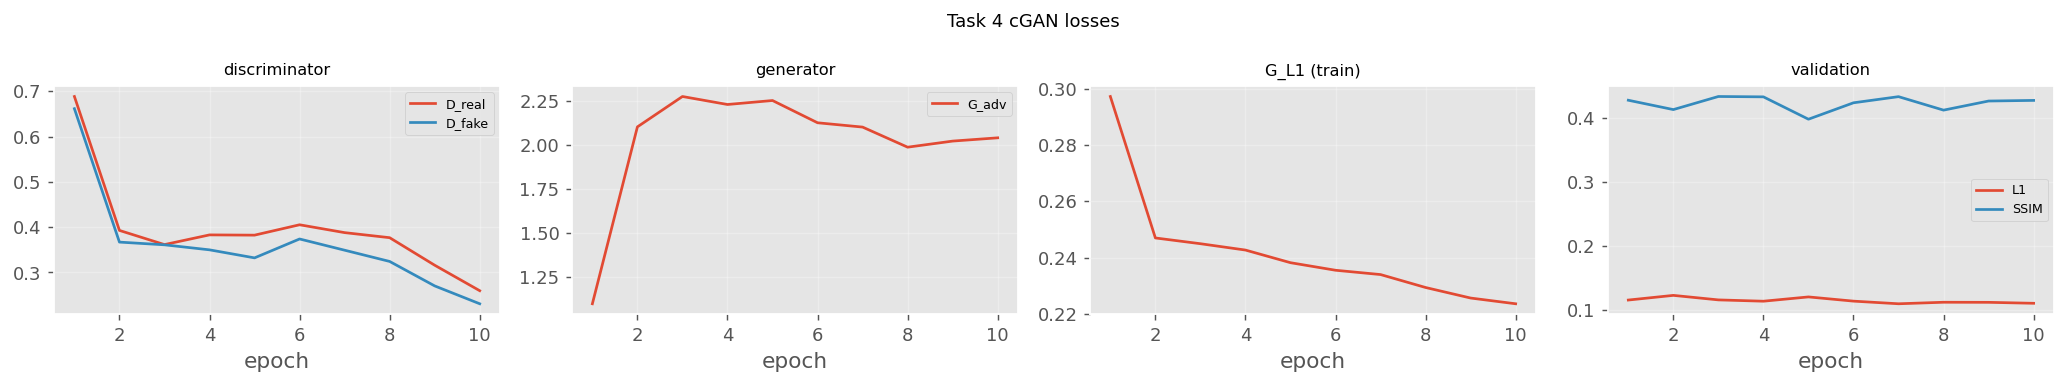
\includegraphics[width=\linewidth]{task4_curves}\caption{Task 4 losses: D-real, D-fake, G-adversarial, G-$L_1$ and validation metrics.}\label{fig:t4loss}\end{figure}
\begin{figure}[t]\centering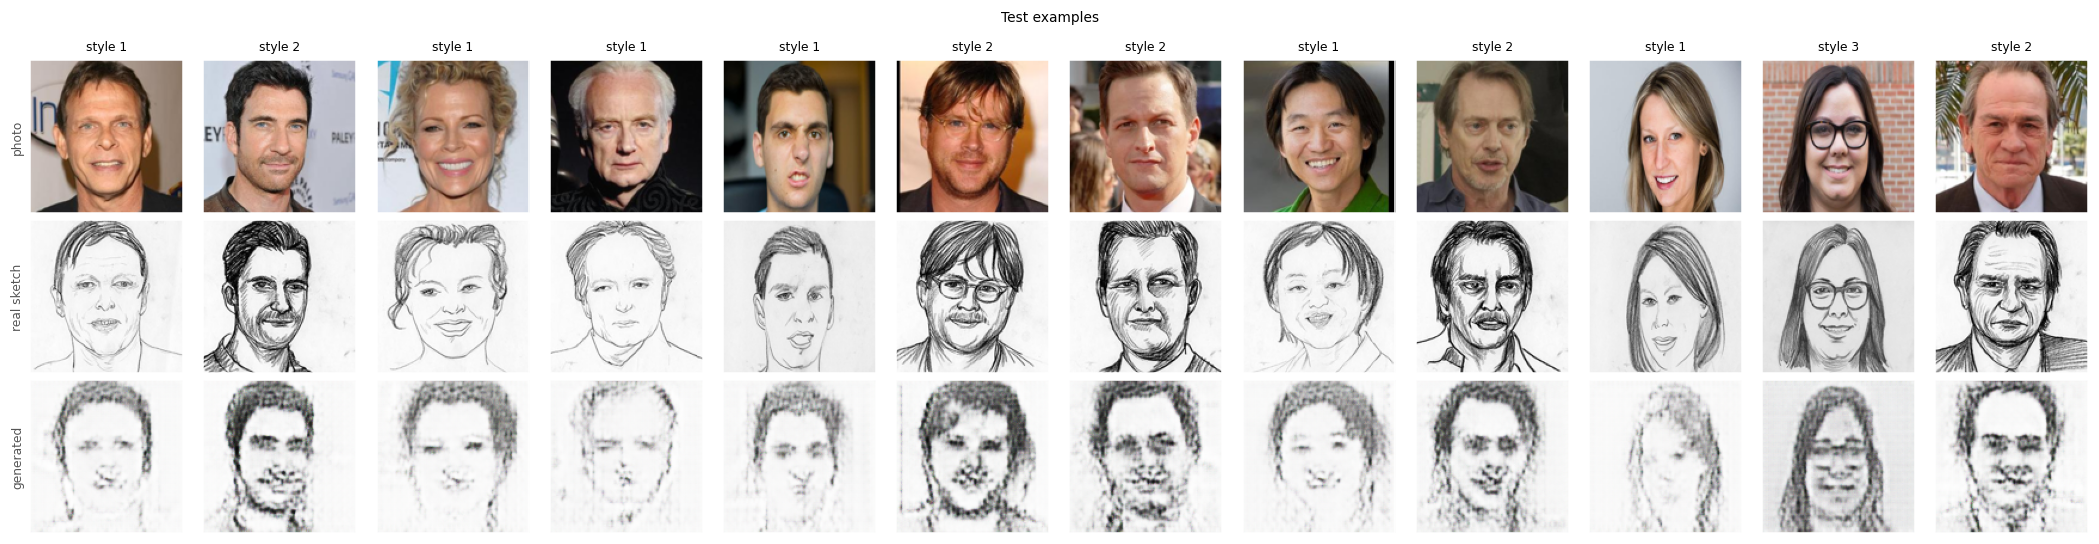
\includegraphics[width=\linewidth]{task4_test_examples}\caption{Task 4 test examples: photo, real sketch, generated sketch.}\label{fig:t4ex}\end{figure}
\begin{figure}[t]\centering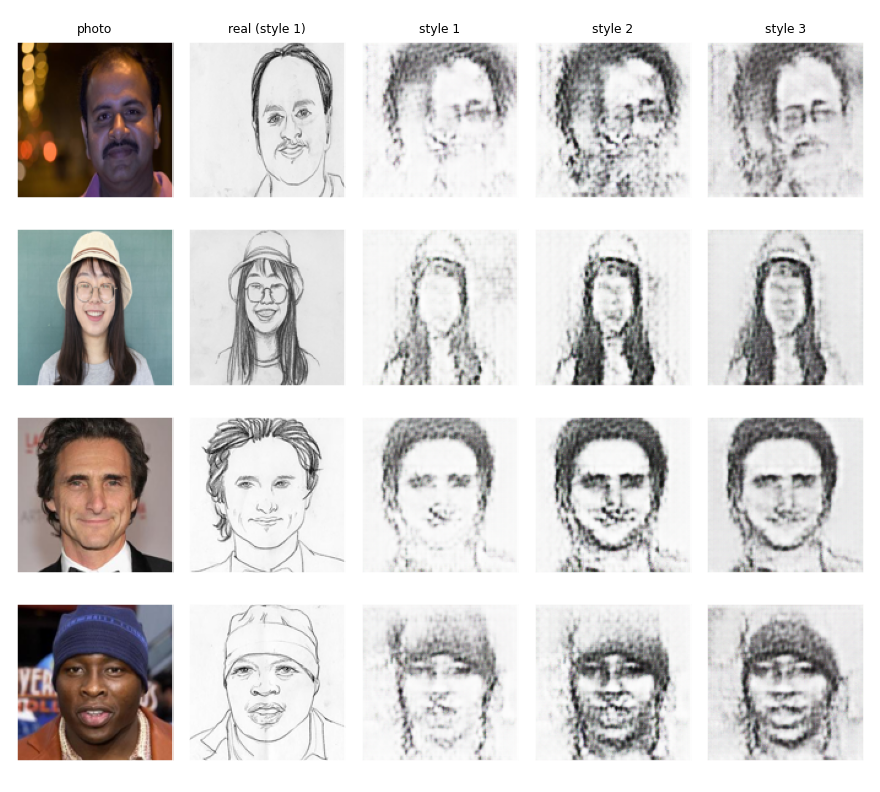
\includegraphics[width=\columnwidth]{task4_style_control}\caption{Style control: one photograph rendered in Styles 1--3.}\label{fig:style}\end{figure}
\begin{figure}[t]\centering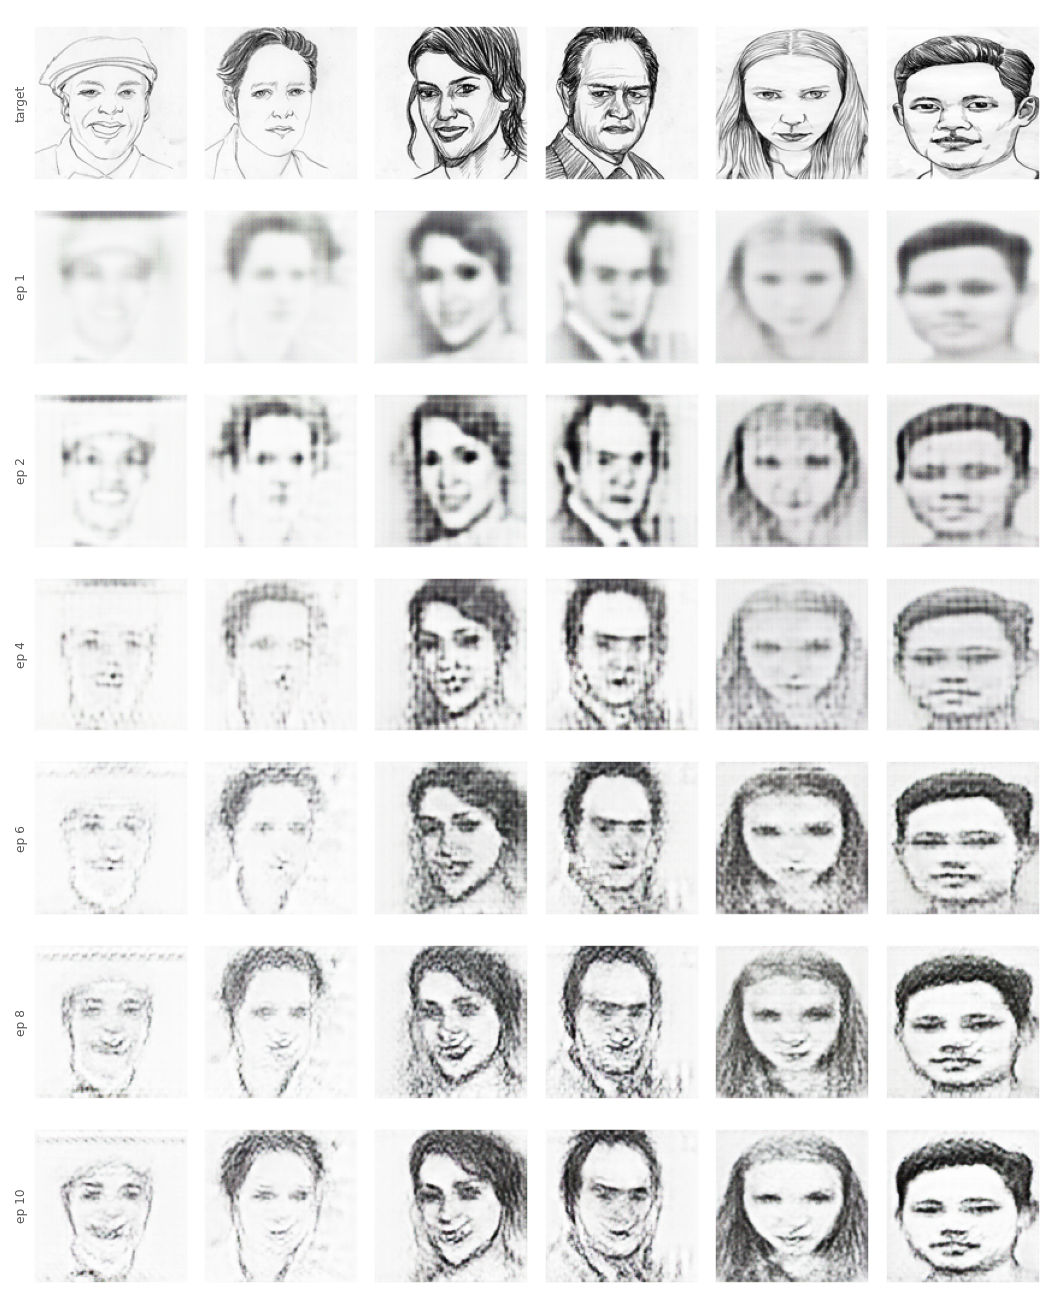
\includegraphics[width=\columnwidth]{task4_progression}\caption{Generated sketches for the same validation photographs during training.}\label{fig:prog}\end{figure}
\begin{figure}[t]\centering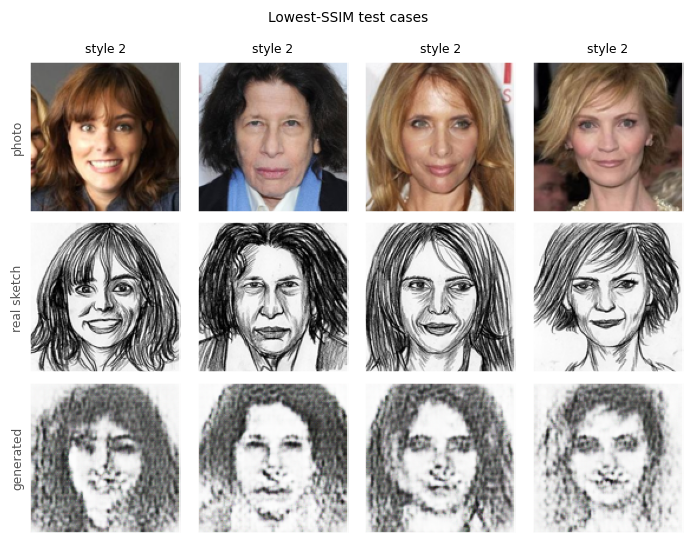
\includegraphics[width=\linewidth]{task4_failures}\caption{Task 4 lowest-SSIM test cases.}\label{fig:t4fail}\end{figure}


%=====================================================================
\section{ONNX Export and Verification}
All seven inference models (universal DAE, classifier with softmax, three specialists, complete soft-MoE pipeline returning output, weights, logits and branch outputs, and the generator with an \texttt{int64} style input) are exported with opset 17 and dynamic batch size. Each is run in ONNX Runtime on real corrupted test images and compared with PyTorch. During development the classifier initially showed a 0.74 discrepancy: \texttt{torch.onnx.export} restores the previous train/eval flag of the \emph{wrapper} module on the whole tree, putting BatchNorm back into training mode for the PyTorch reference. Forcing \texttt{eval()} before verification removed the discrepancy; the ONNX graph itself was correct.

The export script writes the per-output differences to \texttt{outputs/tables/onnx\_verification.csv}; for the trained models all seven agreed with PyTorch, with a maximum absolute difference of $1.0\cdot10^{-5}$ (soft-MoE output and occlusion specialist) and below $10^{-6}$ for the classifier probabilities and routing weights.

%=====================================================================
\section{Application}
The interface (four workspaces plus a System page) was first designed in Google Stitch and implemented in React with Tailwind CSS. A FastAPI backend validates uploads (type, size, decodability), resizes to 128$\times$128, applies optional runtime corruption with the training code, runs ONNX Runtime and returns images, metrics (PSNR/SSIM when a clean reference exists), error maps, routing probabilities or mixture weights and per-component inference times. Endpoints: \texttt{/api/health}, \texttt{/api/corrupt}, \texttt{/api/restore/\{universal,hard,soft\}}, \texttt{/api/sketch}. Docker Compose starts the backend, an nginx-served frontend and an MLflow UI with \texttt{docker compose up --build}.

% Put screenshots in figures/ and uncomment:
% \begin{figure}[t]\centering\includegraphics[width=\columnwidth]{stitch_design}\caption{Original Google Stitch design.}\end{figure}
% \begin{figure}[t]\centering\includegraphics[width=\columnwidth]{app_soft_moe}\caption{Soft MoE workspace with routing weights and expert outputs.}\end{figure}


%=====================================================================
\section{Limitations}
Training ran on a free Colab T4 under a strict deadline. Tasks 1 and 2 used the planned schedule; the Task~2 final retraining, and especially Tasks~3 and~4, used a reduced schedule (few Optuna trials and epochs), so their results are a lower bound rather than converged performance. The dense, skip-free bottleneck limits fine detail (texture is smoothed), which is the intended trade-off of a genuine autoencoder. Optuna for the GAN optimises a reconstruction metric, which favours larger $\lambda_{L1}$ and does not directly measure perceptual realism (FID/LPIPS were not computed). All inference runs on CPU in the container.

\section{Conclusion}
A complete research-to-deployment pipeline was built for four generative systems. Explicit routing with specialists and a near-perfect corruption classifier gives strong, interpretable restoration; the soft MoE makes routing differentiable and can blend experts for ambiguous or mixed corruptions; and a style embedding injected into both generator and discriminator gives categorical control over sketch synthesis. Longer training of Tasks~3 and~4 is the clearest next step.

%=====================================================================
\appendices
\section{AI-Use Statement}
\textbf{Tool:} Claude Code (Anthropic), used as a coding and writing assistant.
\textbf{Used for:} scaffolding the training/evaluation code, Optuna/MLflow integration, ONNX export, FastAPI backend, React frontend and Docker configuration; debugging; drafting this report.
\textbf{Verification and corrections:} every component was executed end-to-end in a CPU Docker smoke test before GPU training; corruption parameters were checked numerically against the specification (which exposed and fixed an occlusion-coverage bug, 8.7\%$\rightarrow\geq$10\%); ONNX outputs were compared numerically with PyTorch (which exposed the train/eval-mode bug above); a fresh clone of the repository was tested, which exposed a \texttt{.gitignore} rule that had silently excluded \texttt{src/data}; a DataLoader worker accumulation that killed a Colab run was fixed. Reported numbers come only from the logged experiment outputs. I reviewed the code and am responsible for the submitted system.

\begin{thebibliography}{10}
\bibitem{vincent2008} P. Vincent, H. Larochelle, Y. Bengio, P.-A. Manzagol, ``Extracting and composing robust features with denoising autoencoders,'' ICML, 2008.
\bibitem{unet} O. Ronneberger, P. Fischer, T. Brox, ``U-Net: Convolutional networks for biomedical image segmentation,'' MICCAI, 2015.
\bibitem{ssim} Z. Wang, A. C. Bovik, H. R. Sheikh, E. P. Simoncelli, ``Image quality assessment: from error visibility to structural similarity,'' IEEE TIP, 2004.
\bibitem{zhao2017} H. Zhao, O. Gallo, I. Frosio, J. Kautz, ``Loss functions for image restoration with neural networks,'' IEEE TCI, 2017.
\bibitem{jacobs1991} R. A. Jacobs, M. I. Jordan, S. J. Nowlan, G. E. Hinton, ``Adaptive mixtures of local experts,'' Neural Computation, 1991.
\bibitem{shazeer2017} N. Shazeer et al., ``Outrageously large neural networks: The sparsely-gated mixture-of-experts layer,'' ICLR, 2017.
\bibitem{switch} W. Fedus, B. Zoph, N. Shazeer, ``Switch Transformers,'' JMLR, 2022.
\bibitem{pix2pix} P. Isola, J.-Y. Zhu, T. Zhou, A. A. Efros, ``Image-to-image translation with conditional adversarial networks,'' CVPR, 2017.
\bibitem{fs2k} D.-P. Fan et al., ``Facial-sketch synthesis: A new challenge,'' Machine Intelligence Research, 2022.
\bibitem{optuna} T. Akiba et al., ``Optuna: A next-generation hyperparameter optimization framework,'' KDD, 2019.
\bibitem{parkhi} O. M. Parkhi, A. Vedaldi, A. Zisserman, C. V. Jawahar, ``Cats and dogs,'' CVPR, 2012.
\end{thebibliography}

\end{document}
